\documentclass[onecolumn]{article}
\usepackage{CJKutf8, graphicx}%导入CJKutf8包,并且激活中文、日文、韩文的uft8编码
\usepackage[utf8]{inputenc}
\usepackage{setspace}
\renewcommand{\baselinestretch}{1.5}

\title{短视频传输实验报告}
\author{计研173 \quad 陈雨兰 \quad 2017310787  \\ 计研173 \quad 蔡文静 \quad 2017210866}
\date{January 2018}

\begin{document}
\begin{CJK*}{UTF8}{gbsn}

\maketitle
\section{介绍}
该项目实现了从客户端到服务器端的短视频的快速上传。我们在UDP协议传输数据的基础上加上了数据解压缩、差错控制和数据包校验,实现了短视频的快速准确的传输。

\section{项目设计与分析}
\subsection{算法框架}
为了应对UDP传输中的丢包和乱序的情况,我们采用前向纠错技术进行丢包恢复。
该算法由发送方进行FEC编码引入冗余包,接收方进行FEC解码并恢复丢失的数据包。
对于包乱序和包重复,我们采用QOS乱序恢复处理,该QOS方案特点是在没有丢包的情况下,不引入任何系统延时,并且可以通过可控的丢包等待时延来适应不同的信道乱序程度。
QOS需要在接收端进行FEC解码前进行,确保送FEC解码模块的数据包序号是正确的(不存在乱序,仅存在丢包)。
图1为算法的主要框架。

\begin{figure}[h]
	\centering
	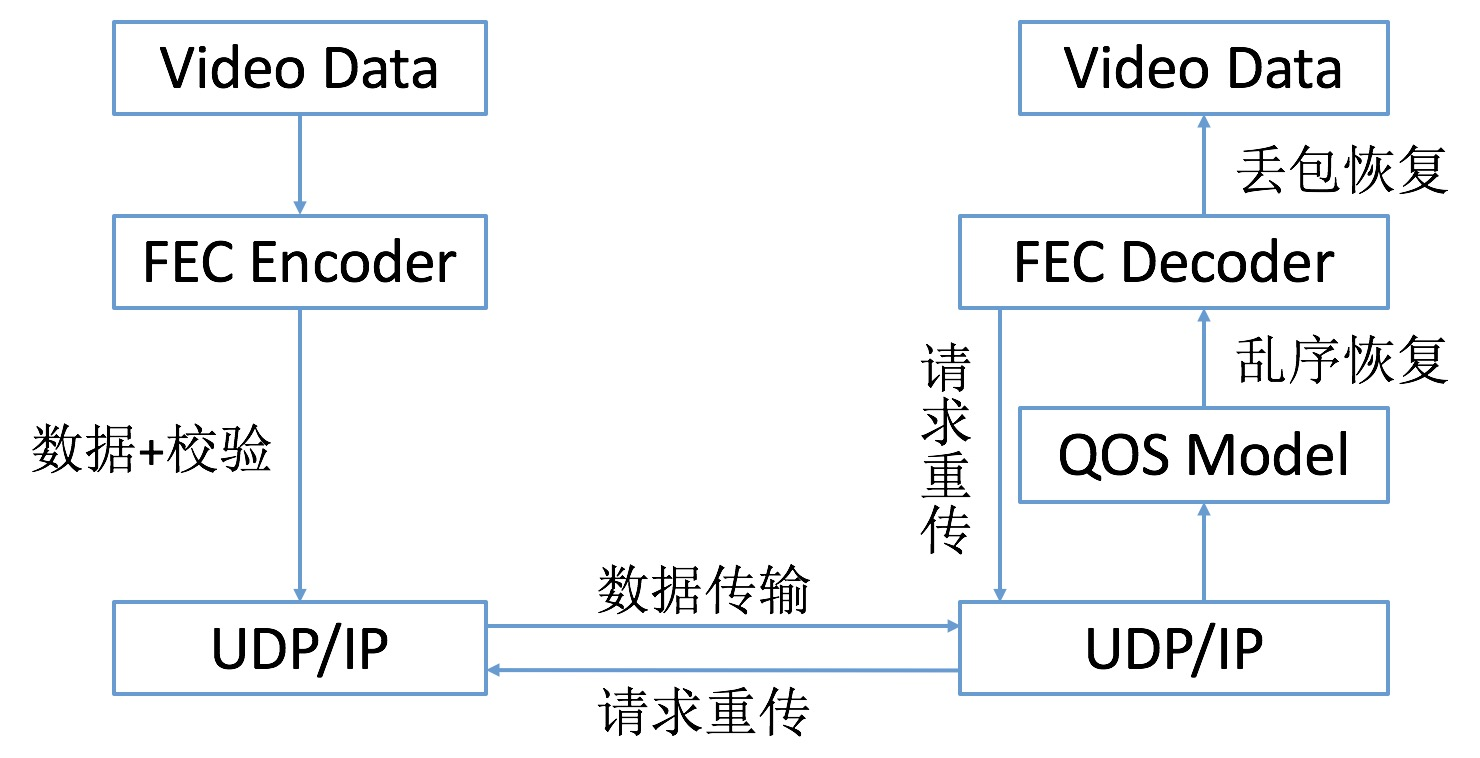
\includegraphics[width=4in]{frame.jpg}
	\caption{算法框架}
	\label{fig:frame}
\end{figure}

本算法侧重于优化具备随机信道特性的传输链路,即连续丢包的概率远低于单包丢失的情况。
当丢包率超过前向纠错的恢复上限时,算法无法恢复所有数据,此时若要保证传输的正确性,需要引入请求重传机制。

\subsection{传输协议}
TCP和UDP是比较常用的传输协议。TCP提供可靠的通信传输,而UDP则常被用于让广播和细节控制交给应用的通信传输。
\subsubsection{TCP协议}
TCP是一种面向连接的协议,能提供可靠的传输服务,即TCP通过检验和、序列号、确认应答、重发控制、连接管理以及窗口控制等机制实现可靠性传输。TCP充分实现了数据传输时各种控制功能,可以进行丢包的重发控制,还可以对次序乱掉的分包进行顺序控制。但是这些功能也限制了TCP数据传输的速度,而且使得系统资源要求较高。
\subsubsection{UDP协议}

UDP是一个非连接的协议,传输数据之前源端和终端不建立连接,当它想传送时就简单地去抓取来自应用程序的数据,并尽可能快地把它扔到网络上。在发送端,UDP传送数据的速度仅仅是受应用程序生成数据的速度、计算机的能力和传输带宽的限制;在接收端,UDP把每个消息段放在队列中,应用程序每次从队列中读一个消息段。由于传输数据不建立连接,因此也就不需要维护连接状态,包括收发状态等,因此一台服务机可同时向多个客户机传输相同的消息。UDP信息包的标题很短,只有8个字节,相对于TCP的20个字节信息包的额外开销很小。UDP使用尽最大努力交付,即不保证可靠交付,因此主机不需要维持复杂的链接状态表(这里面有许多参数)。UDP是面向报文的。发送方的UDP对应用程序交下来的报文,在添加首部后就向下交付给IP层。既不拆分,也不合并,而是保留这些报文的边界,因此,应用程序需要选择合适的报文大小。

基于上述分析,TCP和UDP分别有如下几个特点:
\begin{itemize}
\item TCP面向连接;UDP面向无连接
\item TCP面向字节流;UDP面向报文
\item TCP首部开销大,有20字节,且占用资源较多;UDP首部开销小,只有8字节,且占用资源少
\item TCP提供可靠的服务,即,通过TCP连接传送的数据,无差错,不丢失,不重复,且按序到达;UDP尽最大努力交付,即不保证可靠交付;
\item UDP发送数据速度更快
\end{itemize}

\subsection{丢包恢复}
\begin{figure}[h]
	\centering
	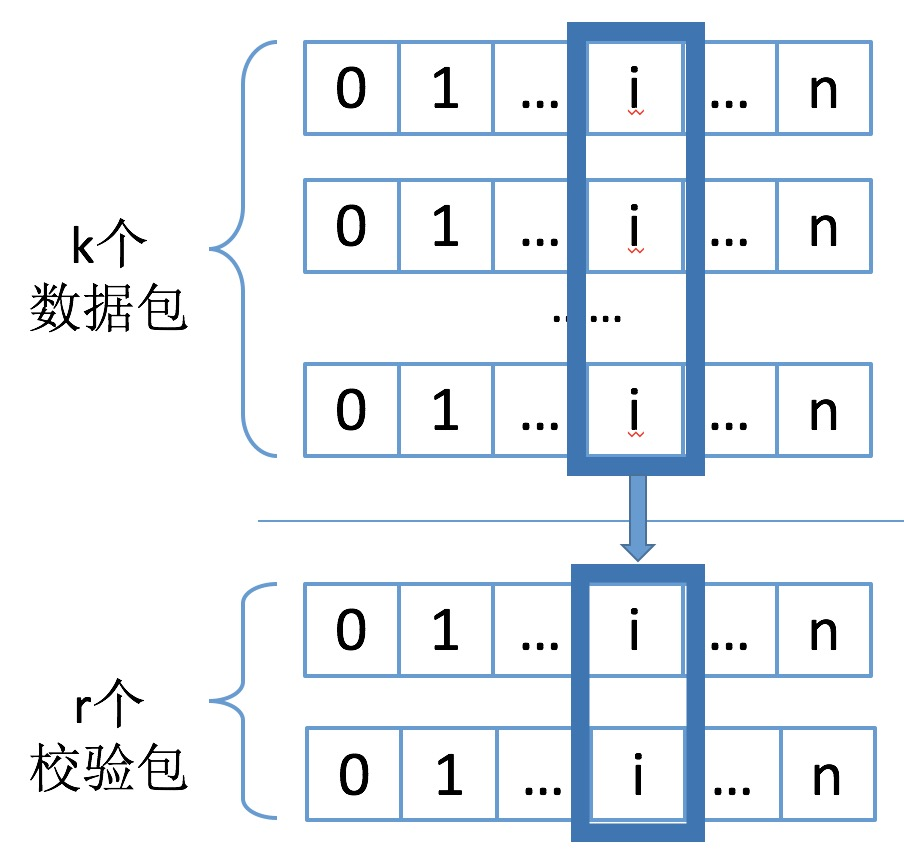
\includegraphics[width=2in]{FEC.jpg}
	\caption{前向纠错算法}
	\label{fig:FEC}
\end{figure}

前向纠错(FEC)技术近年来广泛应用于信息处理的各个领域。
FEC算法通过主动提高冗余度来降低丢包重传的频率,从而降低传输延时。

本次实验中的FEC算法在应用层实现,以数据包为单位进行丟包检测与丟包恢复。
UDP协议保障了包内数据的正确性,我们无需考虑包内纠错,只处理包丢失的情况。
每k 个数据包可以生成r个冗余包,共同构成一个组,即为一个独立的处理单元。
组内每个包拥有连续的编号,通过读取编号可以判断数据包的丟失情况,并予以恢复(冗余包丟失无需恢复)。 

由于冗余性的存在,一个组中任意k个包可以用来重建原始的k个数据包。
如果丟失数据包数小于或等于r,接收者收到一个Group中任意的k个数据包后,即可以通过组号信息确定丟失包的相对位置并进行FEC解码,恢复k个原始媒体包。
这里我们定义冗余包数r与原始媒体包数k的比值为FEC编码冗余度,冗余度越高,抗丟包能力越强,同时传输效率也越低。
找到传输效率与抗丟包能力二者的折中,从而 选择合适的冗余度配置是本方案实际应用过程中必须考虑的问题。

实验中采用Vandermonde矩阵RS算法,下面对算法进行简述:

 (1)数据包分割
 
对数据包进行FEC编码运算首先进行的是包内分割,将数据包分割为多个定长单元,定长单元称为字,设字长为wbits,w的取值一般为8、16、或者32。FEC编码对 k个原始媒体包逐字进行处理,生成m个冗余数据包中与之对应的字。例如现有两个 原始数据包Dl、D2,包的长度都为b bytes (对于包长不足b bytes的使用0补齐), 字长为wbits,那么一个数据包的总字长为l=8b/w。用这两个数据包产生两个冗余包 Cl、C2的过程简述如下:

(2) Vandermonde编解码以及改进

设k个原始数据包为$D= (D_1,D_2,\dots,D_k)$,r个冗余包为$C=(C_1,C_2,\dots,C_r)$,那么传输组可以表示为$Y= (D,C)$。
B 为rxk维FEC生成矩阵,则冗余包生成满足:

$$C=BD$$

在接收端,如果接收者收到了 Group中的任意k个数据包,即可根据所收到的数据包在组中的位置,从FEC生成矩阵B中提取对应的行, 组成一个新的kxk维矩阵B’,显然

$$Y'=B'D$$

如果B’为非奇异矩阵,那么就可以通过如下逆变换得到原始数据包,完成恢复。

$$D=(B')^{-1}Y'$$

设计RS码的关键在于怎样设计生成矩阵B,也就是其系数矩阵G。本方案使用Vandermonde矩阵来构建系数矩阵G。
常规定义Vandermonde矩阵V,r*k维,如下 所示:

$$V=
	\left[ \begin{array}{ccccc}
	1      & 1      & 1      & \cdots & 1       \\
	1      & 2      & 2^2    & \cdots & 2^{k-1} \\
	\vdots & \vdots & \vdots & \ddots & \vdots  \\
	1      & r      & r^2    & \cdots & r^{k-1}
	\end{array} 
	\right ]$$

系数矩阵G=V,该矩阵元素的运算都是在有限域$GF(2^8)$中进行的。

\subsection{乱序恢复}
QOS (Quality of Service,服务质量)的广义概念是指一个网络能够利用各种基础技术,为指定的网络通信提供更好的服务能力。
本方棄中的QOS是指狭义的QOS, 特指用来解决RTP (UDP)传输在不可靠线路(尤其4G、3G、WIFI)下网络包乱序、 包重复、包延时抖动问题的一种技术。

RTP协议头部的包序号为我们进行乱序重排以及重复包丢弃提供了理想的参考值。
正常情况下,包序号逐包递增。本方案通过对接收的数据包进行局部缓存并排序,同时去除接收的重复包以及超时包,最大限度保证接收质量。
本方案相比普通的排序方棄优势在于“边排序边输出”,而不是简单的“先排序后输出”。
在没有丢包的情况下,后者也会引入系统延时,而本方棄则仅在出现乱序、 丢包时才会幻入“等待延时”,这种等待延时是实现QOS无法避免的。

经过QOS处理后的数据包按包序号从小到大输出给后面的FEC解码环节,后者进行丢包的恢复,二者相互配合,各司其职。
方案使用环形队列作为数据结构,通过“条件插入”与“周期取包”实现所需功能。 其中,前者负责将输入包放到合适的位置或做丢弃处理,后者“周期取包”是外部触发的,对队列进行扫描并输出满足条件的包的过程。

新到数据包根据其序号和人列中已有序号进行对比,计算出其存放位置,设为新到包位置,Pout为即将输出的第一个数据包位置,以为新到包的包序号, 为即将输出的第一个数据包包序号,Qgigg为整个环形队列大小,则:
$$Pnew = (Pout + (Nnew - Nout))\%Qsize$$
找到位置后,首先判断该位置是否已经存在数据包,如果存在,则说明当前包是重复包,直接丢弃,以此消除重复包。下面结合示意图说明:
由此可见,“丢包时延”是一个非常重要的QOS参数,如果丢包时延设置得过小, 系统抵御乱序的能力变弱。
如果“丢包时延”设置得过大,则丢包发生时,系统等待延时变大。

\subsection{请求重传}
ACK是大家比较熟悉的传输层保障措施,在类TCP的UDP传输方案中(UDT、KCP等)中通过优化ACK发送时机、更短的超时重传时间等措施来获得更高的数据吞吐率,但ACK并不适合对实时要求极高的直播互动领域。

NACK与ACK不同,它是在没有收到数据包时向远端请求重传,因而更加适合实时通讯。通过与FEC的结合,只对FEC无法恢复的数据包请求NACK重传,能够尽量的降低重传发起概率,降低重传带来的副作用。

NACK可以放置在原来的FEC-QOS传输层之外,作为上层应用层,这种实现方式NACK将FEC-QOS看做普通的UDP传输,二者并无紧密结合,其优势是可以与成熟的NACK方案无缝衔接。我们知道任何NACK方案都必将引入延时抖动,因为接收端在发起重传请求后,需要等待发送端重新发出的数据,在“重传等待时间”内不对外输出数据。而QOS阶段里为解决UDP乱序包的问题也引入了一个“丢包等待时间”,当遇到包序号不连续时,将等待这一时间,若仍未收到所需的包则认定丢包,不再等待。如果将这两个时间合二为一,可以尽量的降低系统时延和抖动,毕竟我们需要的是一个高实时性的NACK传输方案。我们将NACK的发起和等待放置在QOS之中,入下图所示:

当QOS检测到序号不连续时,可能是发生丢包或者是乱序,此时QOS将通过FEC解码模块分析当前疑似丢包是否将导致FEC无法恢复。此时将产生三种分析结果:

A、当前丢包即使丢了也不影响FEC恢复,比如当前丢失的包为一个或者多个冗余包,且该冗余包所在的group内的媒体包均已接收,或者借助已接收的冗余包足够恢复。

B、当前丢包不能确定是否影响FEC恢复,需要接收更多的包才能确定。比如丢包发生在group的中段且丢的数量小于冗余包总数。

C、当前丢包将导致FEC确定无法恢复,比如同一个group内丢失的包数大于冗余包总数。

对于情况A,QOS将直接不予等待,将后续接收的包直接交与FEC。对于情况B,QOS将进入“丢包等待时间”,以期收到乱序的包。对于情况C,QOS将发起NACK重传并进入等待,这个等待时间即是“丢包等待时间”又是“重传等待时间”,在等待期内不管是该乱序包到达或者重传包到达,都能满足FEC的恢复条件。

在介绍了NACK的发起条件后,我们来关注“重传等待时间”的取值问题。若设置固定的重传等待时间将很难满足各类网络情况。时间过小将导致重传包尚未到达,QOS已结束等待并输出后续包,后续即便再收到重传包也将直接丢弃。重传包也可能因网络原因丢包,若“重传等待时间”过大,将导致更大的延时和抖动。为了提高自适应能力,系统通过实时获取当前网络的UDP通讯RTT时间来作为“重传等待时间”的参考,计算出合理的值。

我们使用独立的一个UDP信令通道用来传输NACK请求,而不是复用媒体通道。这样做的主要考虑是:

A、媒体通道上使用的FEC/QOS将必然引入部分延时和抖动(具体参见FEC/QOS原理说明),NACK请求对于时间特别敏感,希望是越早越快通知对方越好。在信令通道上我们将只进行裸UDP收发,不会加入FEC和QOS。

B、避免出现NACK请求包丢失后也发起NACK重传请求的情况。

C、更好的兼容性,对于不支持NACK的节点,只需要忽略信令通道的内容即可与NACK节点互通。

D、程序实现上更加简洁,无需在媒体通道上新增包类型来区分哪个包是NACK请求包。媒体包上增加字节也都会直接转化为带宽的增长。

对于传输层模块,它是全双工的,为演示方便我们只列出单向的情况,另外一个方向也是完全一致的。在FEC编码之后,所有的发出的UDP(RTP)包均会被存入一个环形缓存区中,当收到远端NACK请求时,将在下一个媒体包传输时触发重传动作,后者将在环形缓存区中检索需要重传的包并在媒体通道上发出。我们没有新增内部线程去执行重传动作,而是借助原本的媒体包发送行为来触发,这样可以简化设计提高稳定性。

检索过程中我们进行了数据包的合法性校验和时间戳有效性校验,当发现当前时间距离数据包初次发送时间的间隔已经较大时,将放弃重传,因为此时远端极有可能已经退出等待,没有必要再浪费带宽。检索使用的是RTP头中的序号字段,需要考虑序号达到最大值时的跳变动作。

\section{项目实现}
我们使用eclipse进行android开发,使用java的socket编程实现udp协议的数据传输。
\begin{figure}[h]
	\centering
	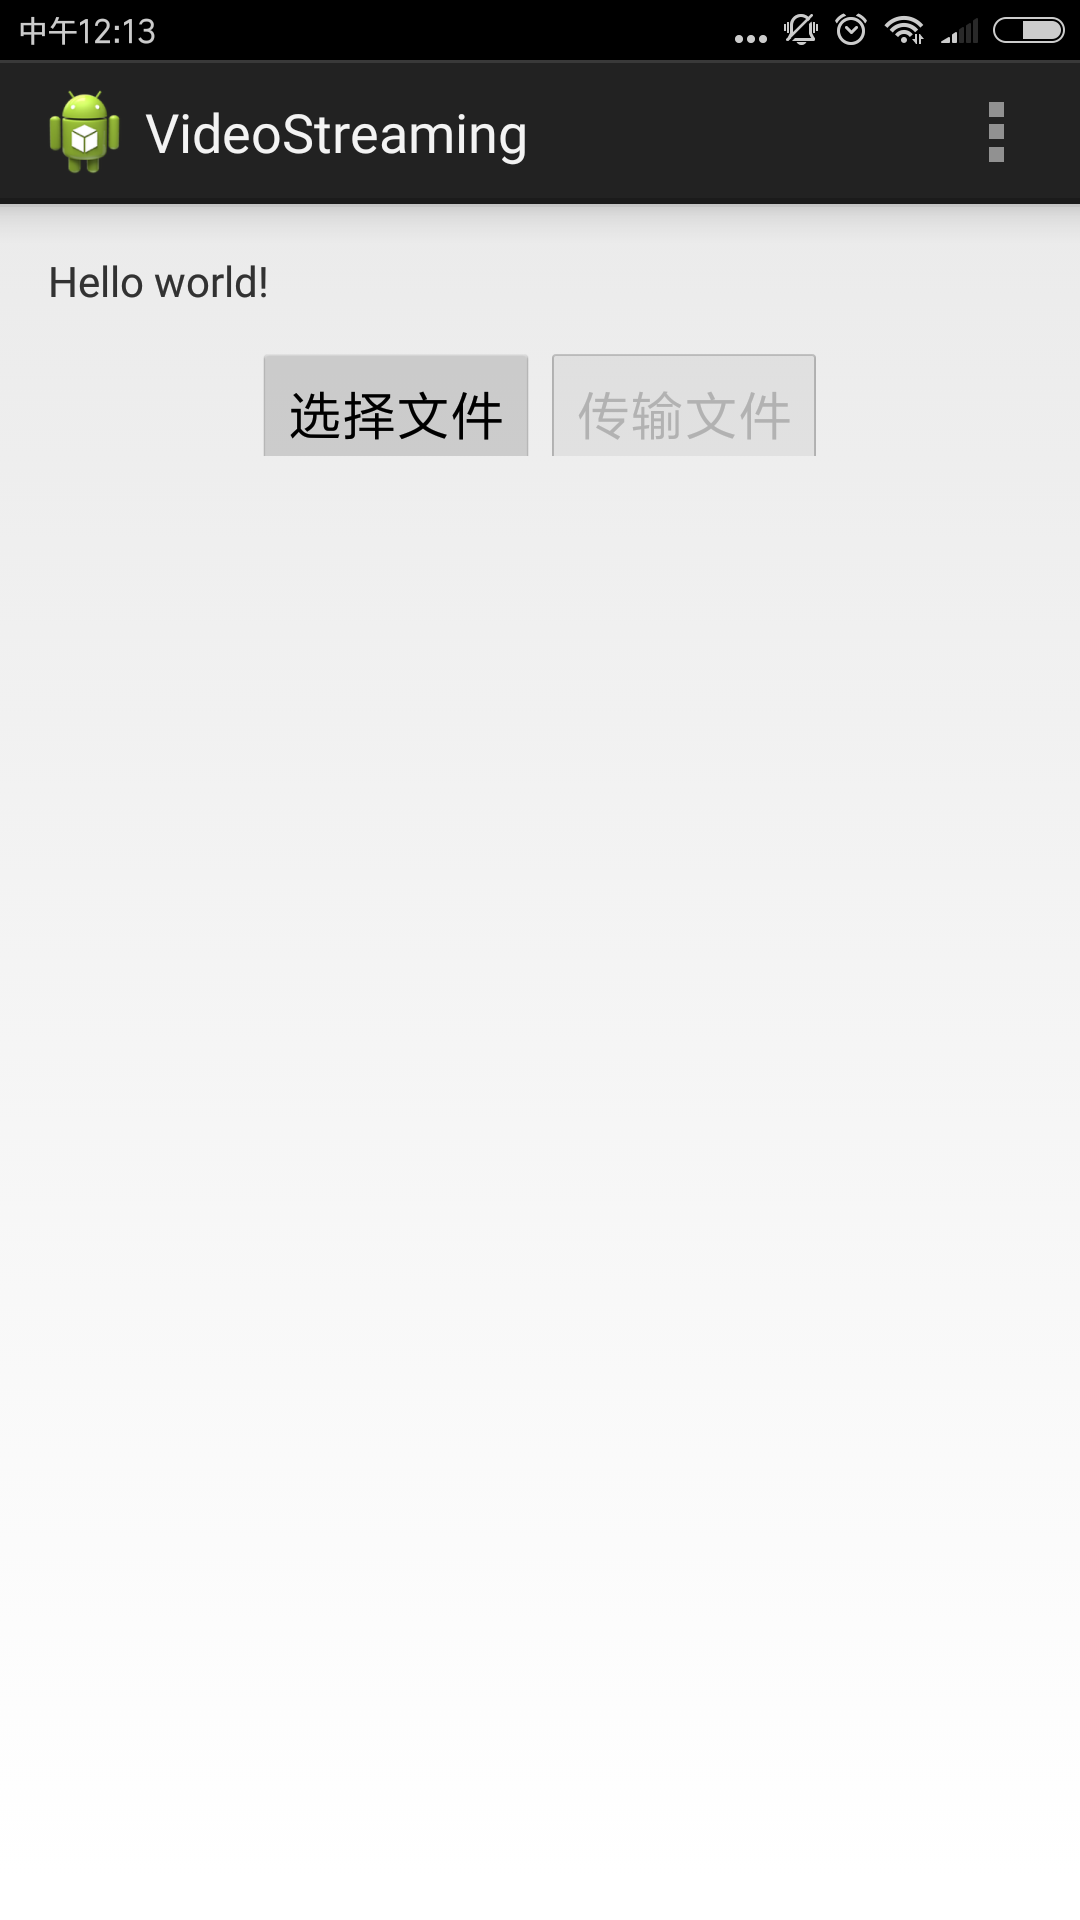
\includegraphics[width=2in]{select.png}
	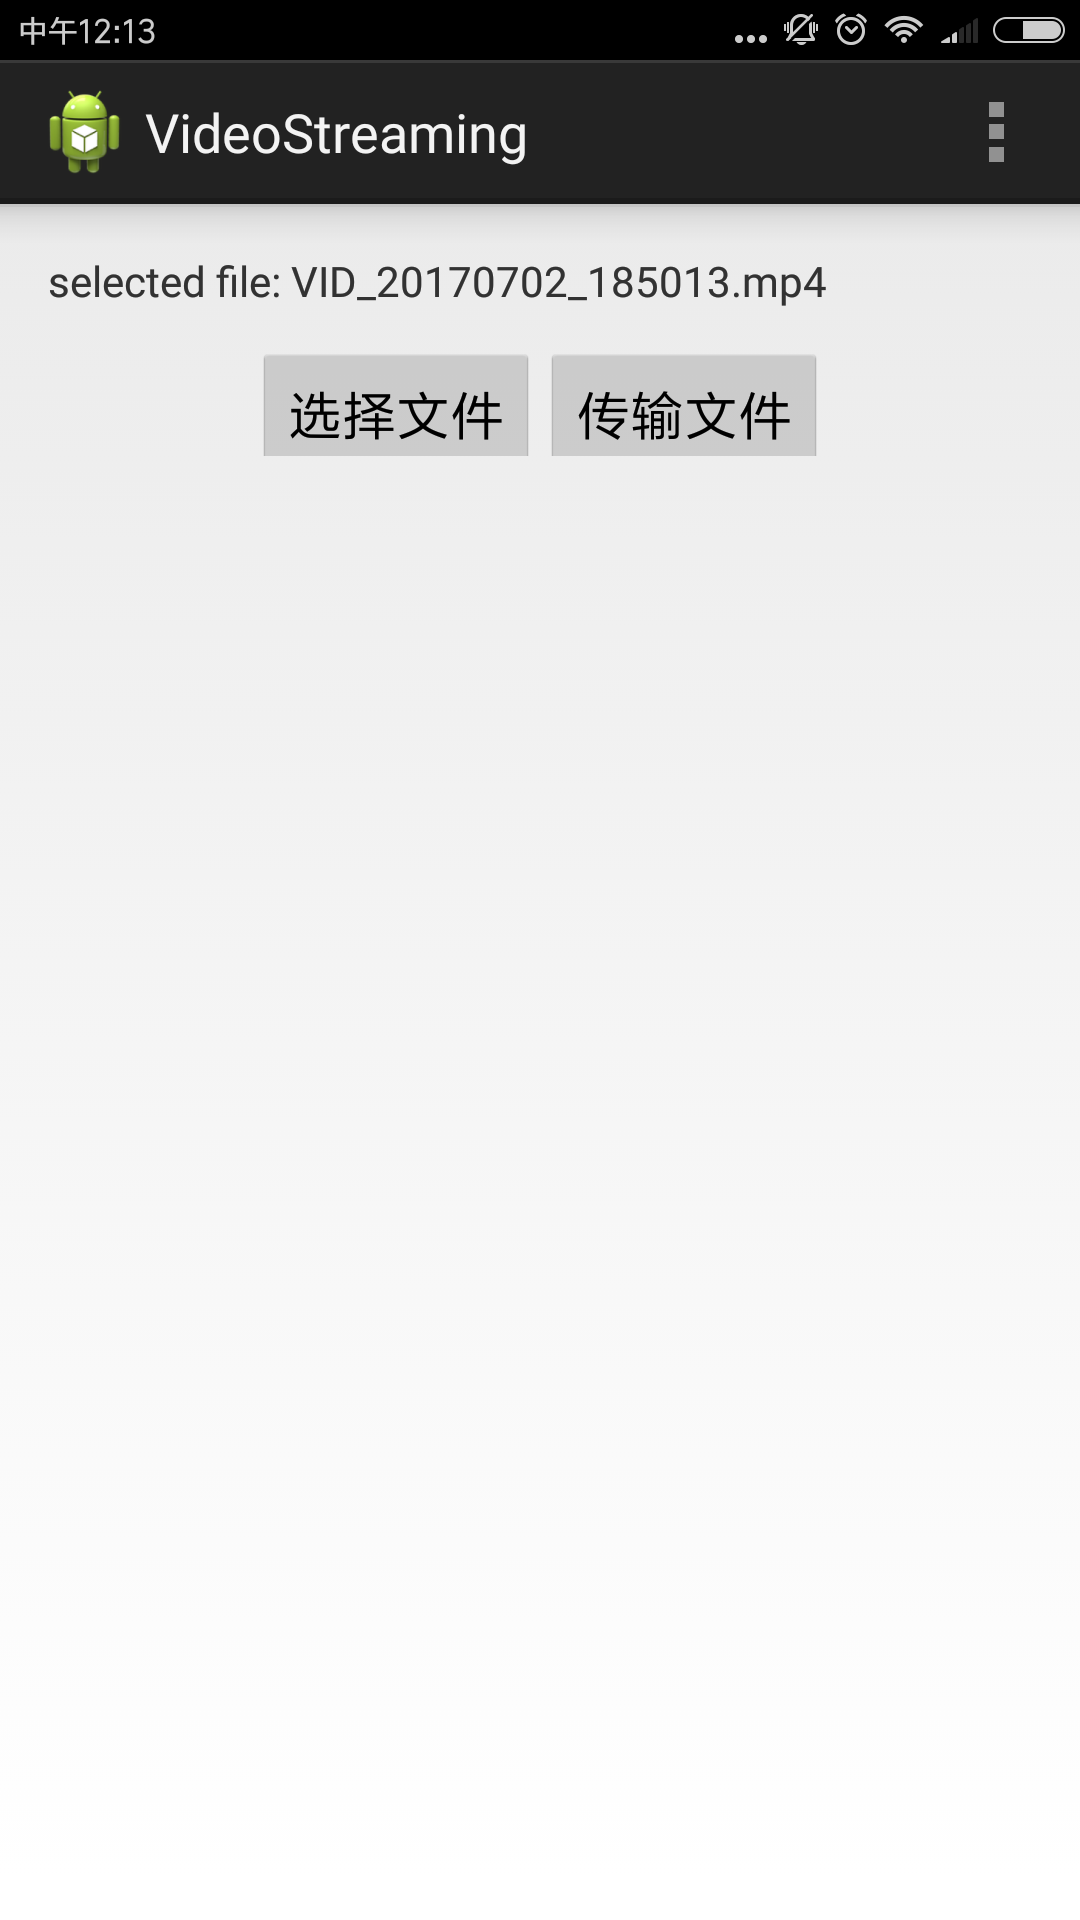
\includegraphics[width=2in]{send.png}
	\caption{android端程序界面}
	\label{fig:android}
\end{figure}

\subsection{实验环境}
\begin{itemize}
\item android. 客户端在android手机上实现了一个应用程序。该程序具有选择文件和传输文件的功能,界面图如图~\ref{fig:android}所示,点击“选择文件”按钮选择想要上传的文件,选择文件后,点击“传输文件”,即开始进行文件上传。\textbf{android测试环境是小米5手机,android 7.0;该应用程序要求android版本最小是andorid 6.0}。


在点击“选择文件”按钮时,我们使用android自带的文件选择器进行文件的选择,这时会出现一个文件选择的目录,选择一个短视频,确定即回到主界面;之后我们要获得被选择文件的路径以便后续使用。在文件选择时,android6.0和以前不一样的地方在于,请求文件之前要再次申请权限,仅仅在AndroidManifest.xml文件中申请是不行的。当有文件被选择时,“传输文件”按钮被激活,点击该按钮,主程序会开启一个线程用来传输文件。该线程首先传输一个编号为0的数据包,该数据包的功能是向服务器端传输文件的信息,包括文件大小和文件名。该数据包的前两个字节表示该包的编号(一般设为0),之后四个字节表示文件大小,其他字节表示文件名。客户端发送该数据包之后会等待服务器端的特定信号(成功信号),收到该成功信号之后,客户端会继续传输文件内容;文件内容的包的前两个字节表示的是编号,该编号从1开始,递增至最大(两个字节是足够表示的)。传输文件结束,客户端会发送退出(exit)信号,在收到服务器端的成功回复后(此时服务器端也退出),客户端退出。在传输文件内容过程中,服务器端发现有丢包时,会向客户端发送重传请求,客户端收到重传请求后会暂停目前数据的传输,先重传缺失的包。

\item 服务器端。服务器端的实现是一个eclipse java程序。测试环境是windows 10 64位。在进行文件传输之前,需要先运行服务器端代码,服务器端即进行特定端口的监听,等待数据包的到来。 
\end{itemize}

\section{实验结果与分析}
\subsection{传输速度与冗余}
由于使用了前向纠错,算法的冗余度基本相当于前向纠错中校验包的比例。
\subsection{丢包修复能力}
在视频传输中,以固定比例随机丢包,测得算法的丢包比例和修复率之间的关系。
\end{CJK*}

\end{document}
